% fig_ejer1d_sum.tex — Factores de x4(t) = u(t)·u(2-t)
\documentclass[tikz]{standalone}
\usepackage{pgfplots}
\usepgfplotslibrary{groupplots}
\pgfplotsset{compat=1.18}
\definecolor{utnblue}{RGB}{0,102,204}
\definecolor{utnred}{RGB}{204,0,0}

\begin{document}
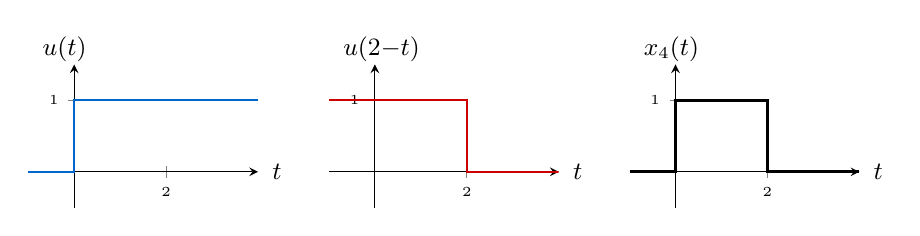
\begin{tikzpicture}
    \begin{groupplot}[
        group style={group size=3 by 1, horizontal sep=0.9cm},
        width=4.5cm, height=3.4cm,
        axis lines=middle,
        xmin=-1, xmax=4, ymin=-0.5, ymax=1.5,
        xtick={0,2}, ytick={0,1},
        xticklabel style={font=\tiny}, yticklabel style={font=\tiny},
        every axis plot/.append style={thick},
        every axis x label/.append style={at={(ticklabel* cs:1.02)}, anchor=west, font=\small},
        every axis y label/.append style={at={(rel axis cs:0.02,0.95)}, anchor=south west, font=\small},
    ]
    % Factor 1: u(t)
    \nextgroupplot[ylabel={$u(t)$}, xlabel={$t$}]
    \addplot[utnblue] coordinates {(-1,0)(0,0)(0,1)(4,1)};

    % Factor 2: u(2-t)
    \nextgroupplot[ylabel={$u(2{-}t)$}, xlabel={$t$}]
    \addplot[utnred] coordinates {(-1,1)(2,1)(2,0)(4,0)};

    % Producto
    \nextgroupplot[ylabel={$x_4(t)$}, xlabel={$t$}]
    \addplot[black, very thick] coordinates {(-1,0)(0,0)(0,1)(2,1)(2,0)(4,0)};
    \end{groupplot}
\end{tikzpicture}
\end{document}
